\section{Free-Space Dipole Design and Tuning}

Before studying the effect of the human body, the dipole antenna must first be established as a valid free-space baseline. The initial geometry was based on the theoretical half-wavelength estimate, and the CST model was then tuned so that the return-loss minimum occurred close to the design operating frequency of \(1.120~\mathrm{GHz}\).

\subsection{Initial Free-Space Geometry}

The wearable antenna was first designed and simulated in free space before introducing the human body model. The initial dipole length was selected from the theoretical half-wavelength value at the target frequency,

\[
L_{\lambda/2} = 133.93~\mathrm{mm}.
\]

The dipole was modeled as two PEC cylindrical arms separated by a \(2~\mathrm{mm}\) center feed gap. The wire radius was

\[
a = 0.905~\mathrm{mm}.
\]

Because the dipole was oriented along the \(x\)-axis, the initial arm length was calculated as

\[
L_{\mathrm{arm}}
=
\frac{L_{\lambda/2}-g}{2},
\]

where \(g=2~\mathrm{mm}\) is the feed gap. Therefore,

\[
L_{\mathrm{arm}}
=
\frac{133.93-2}{2}
=
65.965~\mathrm{mm}.
\]

The right and left dipole arms were defined symmetrically about the origin. The discrete port was placed across the center gap.

\begin{table}[htbp]
\centering
\caption{Initial free-space dipole geometry in CST.}
\label{tab:initial-free-space-geometry}
\begin{tabular}{lc}
\hline
\textbf{Parameter} & \textbf{Value} \\
\hline
Total dipole length & \(133.93~\mathrm{mm}\) \\
Feed gap & \(2.00~\mathrm{mm}\) \\
Wire radius & \(0.905~\mathrm{mm}\) \\
Each arm length & \(65.965~\mathrm{mm}\) \\
Right arm \(x\)-range & \(1.000~\mathrm{mm}\) to \(66.965~\mathrm{mm}\) \\
Left arm \(x\)-range & \(-66.965~\mathrm{mm}\) to \(-1.000~\mathrm{mm}\) \\
Port reference impedance & \(50~\Omega\) \\
\hline
\end{tabular}
\end{table}

The initial CST simulation was performed over the frequency range from \(0.7~\mathrm{GHz}\) to \(1.5~\mathrm{GHz}\). The purpose of this first simulation was to check whether the theoretical half-wavelength estimate produced a good impedance match at the design frequency of \(1.120~\mathrm{GHz}\).

\subsection{Initial Free-Space Result}

The initial free-space simulation showed that the antenna was resonant below the target frequency. The minimum return loss occurred at approximately

\[
f_{\min} = 1.020~\mathrm{GHz},
\]

with

\[
S_{11,\min} = -15.630935~\mathrm{dB}.
\]

However, at the target frequency,

\[
f_0 = 1.120~\mathrm{GHz},
\]

the return loss was only

\[
S_{11}(1.120~\mathrm{GHz}) = -6.45269~\mathrm{dB}.
\]

This result indicates that the theoretical half-wavelength length was electrically too long for the practical CST model. The difference is expected because the actual antenna includes finite wire radius, a finite feed gap, and a discrete feed model. Therefore, the physical resonant length is not exactly equal to \(\lambda_0/2\).

\begin{table}[htbp]
\centering
\caption{Initial free-space CST result before tuning.}
\label{tab:initial-free-space-result}
\begin{tabular}{lc}
\hline
\textbf{Quantity} & \textbf{Value} \\
\hline
Initial dipole length & \(133.93~\mathrm{mm}\) \\
Target frequency & \(1.120~\mathrm{GHz}\) \\
Minimum-\(S_{11}\) frequency & \(1.020~\mathrm{GHz}\) \\
Minimum \(S_{11}\) & \(-15.630935~\mathrm{dB}\) \\
\(S_{11}\) at \(1.120~\mathrm{GHz}\) & \(-6.45269~\mathrm{dB}\) \\
\hline
\end{tabular}
\end{table}

The initial free-space return-loss response before length tuning is shown in Figure~\ref{fig:free-space-initial-s11}.

\begin{figure}[htbp]
\centering
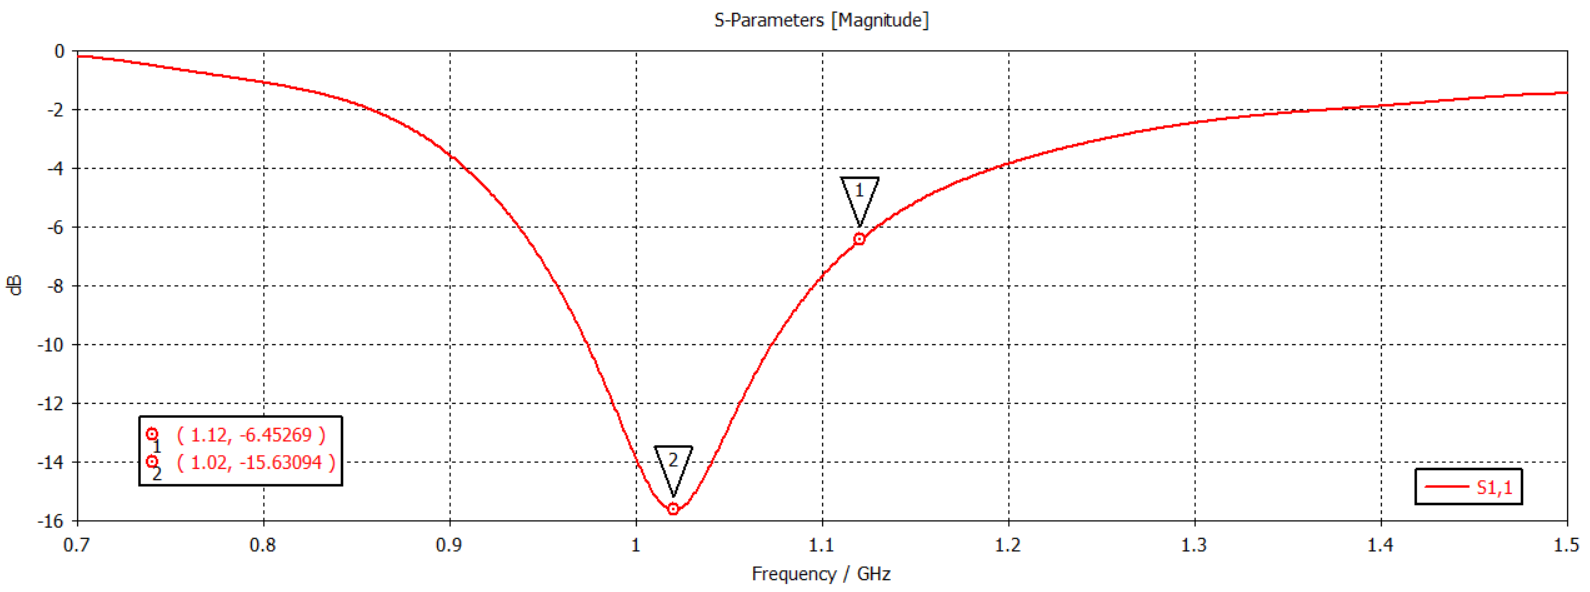
\includegraphics[width=0.82\textwidth]{figures/free_space/s11_free_space_initial_L133p93_with_markers.png}
\caption{Initial free-space return-loss response for the theoretical half-wave dipole length \(L=133.93~\mathrm{mm}\). The minimum occurs at \(1.020~\mathrm{GHz}\), while \(S_{11}\) at \(1.120~\mathrm{GHz}\) is \(-6.45269~\mathrm{dB}\).}
\label{fig:free-space-initial-s11}
\end{figure}

The initial simulation therefore provided the direction for tuning: since the antenna resonated below the target frequency, the dipole length needed to be shortened.

\subsection{Length Tuning}

A first-order tuning estimate was obtained using the approximate inverse relation between resonant frequency and dipole length,

\[
f_r \propto \frac{1}{L}.
\]

The tuned length was estimated from

\[
L_{\mathrm{new}}
=
L_{\mathrm{old}}
\frac{f_r}{f_0}.
\]

Using

\[
L_{\mathrm{old}} = 133.93~\mathrm{mm},
\]

\[
f_r = 1.020~\mathrm{GHz},
\]

and

\[
f_0 = 1.120~\mathrm{GHz},
\]

gives

\[
L_{\mathrm{new}}
=
133.93
\frac{1.020}{1.120}
=
121.99~\mathrm{mm} \approx 122.0~\mathrm{mm}.
\]

This first-order free-space length-retuning calculation is verified using the Python utility script in Appendix~\ref{app:python-utility-calculations}, Listing~\ref{lst:wearable-verification}.

Therefore, the tuned free-space dipole length was selected as

\[
L_{\mathrm{tuned}} = 122.0~\mathrm{mm}.
\]

With the same \(2~\mathrm{mm}\) feed gap, the tuned arm length became

\[
L_{\mathrm{arm,tuned}}
=
\frac{122.0-2.0}{2}
=
60.0~\mathrm{mm}.
\]

Thus, the tuned CST geometry was defined using the following coordinates.

\begin{table}[htbp]
\centering
\caption{Tuned free-space dipole geometry in CST.}
\label{tab:tuned-free-space-geometry}
\begin{tabular}{lc}
\hline
\textbf{Parameter} & \textbf{Value} \\
\hline
Tuned total dipole length & \(122.0~\mathrm{mm}\) \\
Feed gap & \(2.0~\mathrm{mm}\) \\
Wire radius & \(0.905~\mathrm{mm}\) \\
Each arm length & \(60.0~\mathrm{mm}\) \\
Right arm \(x\)-range & \(1.0~\mathrm{mm}\) to \(61.0~\mathrm{mm}\) \\
Left arm \(x\)-range & \(-61.0~\mathrm{mm}\) to \(-1.0~\mathrm{mm}\) \\
Discrete port location & \(x=-1.0~\mathrm{mm}\) to \(x=1.0~\mathrm{mm}\) \\
Port reference impedance & \(50~\Omega\) \\
\hline
\end{tabular}
\end{table}

The tuned free-space geometry used as the baseline model is shown in Figure~\ref{fig:free-space-geometry}.

\begin{figure}[htbp]
\centering
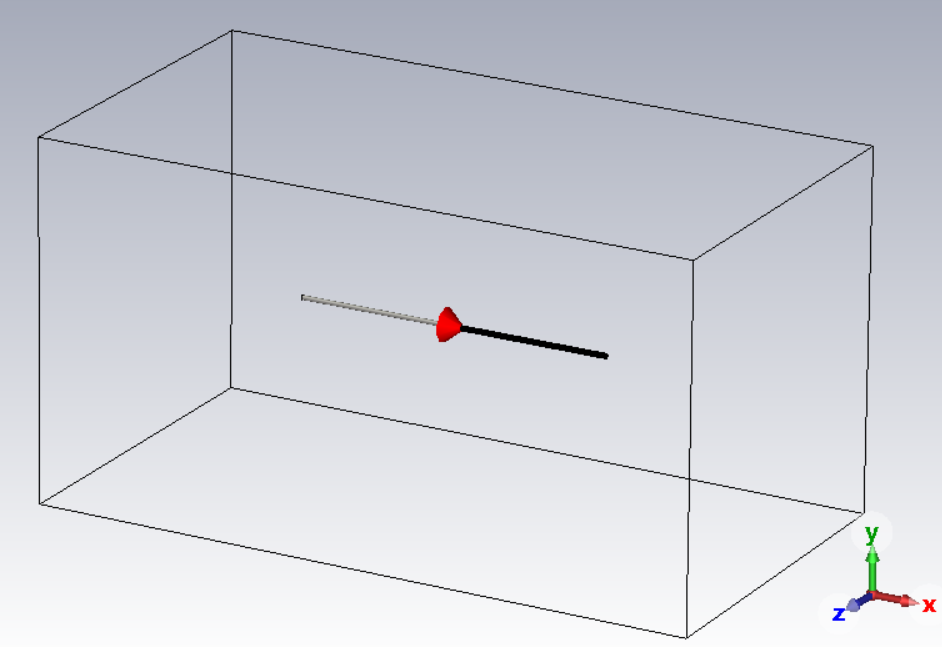
\includegraphics[width=0.82\textwidth]{figures/free_space/geometry_free_space_tuned_L122.png}
\caption{Tuned free-space dipole geometry with total length \(L=122~\mathrm{mm}\), wire radius \(0.905~\mathrm{mm}\), and \(2~\mathrm{mm}\) center feed gap.}
\label{fig:free-space-geometry}
\end{figure}

\subsection{Tuned Free-Space Result}

After shortening the dipole to \(122.0~\mathrm{mm}\), the return-loss minimum moved close to the design target frequency. The tuned free-space result was

\[
f_{\min} = 1.1168~\mathrm{GHz},
\]

with

\[
S_{11,\min} = -15.52702~\mathrm{dB}.
\]

At the target frequency,

\[
S_{11}(1.120~\mathrm{GHz}) = -15.48433~\mathrm{dB}.
\]

This confirms that the tuned free-space dipole is well matched near \(1.120~\mathrm{GHz}\), since the return loss is below the commonly used \(-10~\mathrm{dB}\) matching criterion.

\begin{table}[htbp]
\centering
\caption{Tuned free-space CST result.}
\label{tab:tuned-free-space-result}
\begin{tabular}{lc}
\hline
\textbf{Quantity} & \textbf{Value} \\
\hline
Tuned dipole length & \(122.0~\mathrm{mm}\) \\
Target frequency & \(1.120~\mathrm{GHz}\) \\
Minimum-\(S_{11}\) frequency & \(1.1168~\mathrm{GHz}\) \\
Minimum \(S_{11}\) & \(-15.52702~\mathrm{dB}\) \\
\(S_{11}\) at \(1.120~\mathrm{GHz}\) & \(-15.48433~\mathrm{dB}\) \\
\hline
\end{tabular}
\end{table}

The corresponding tuned free-space return-loss response is shown in Figure~\ref{fig:free-space-s11}.

\begin{figure}[htbp]
\centering
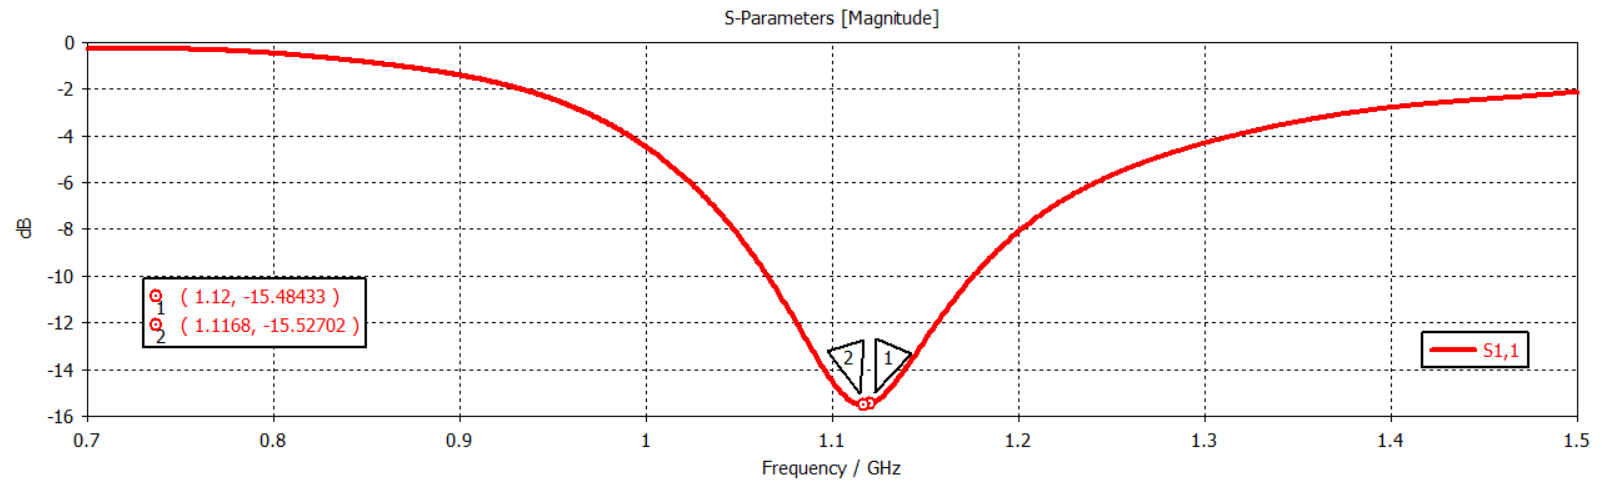
\includegraphics[width=0.82\textwidth]{figures/free_space/s11_free_space_tuned_L122_with_markers.png}
\caption{Return loss of the tuned free-space dipole. The minimum occurs at \(1.1168~\mathrm{GHz}\), and \(S_{11}\) at the target frequency \(1.120~\mathrm{GHz}\) is \(-15.48433~\mathrm{dB}\).}
\label{fig:free-space-s11}
\end{figure}

The tuned free-space antenna was used as the baseline design for all subsequent body-loading simulations. This baseline is important because any later change in \(S_{11}\), gain, radiation efficiency, or radiation pattern can be attributed to the presence and proximity of the lossy multilayer body model.

\subsection{Free-Space Baseline Interpretation}

The free-space simulation demonstrates an important practical antenna-design point. Although the theoretical half-wavelength value gives a useful starting point, the final resonant length must be adjusted in the full-wave model. The final tuned length,

\[
L_{\mathrm{tuned}} = 122.0~\mathrm{mm},
\]

is shorter than the theoretical value,

\[
L_{\lambda/2} = 133.93~\mathrm{mm}.
\]

The percentage reduction is

\[
\frac{133.93-122.0}{133.93}\times 100
=
8.91\%.
\]

This shortening is consistent with the fact that finite-radius dipoles and practical feed models do not resonate exactly at the ideal \(\lambda_0/2\) length. Once tuned, the antenna achieved good matching at the design frequency and could be used as a valid reference for the wearable antenna study.
